\documentclass[11pt,a4paper]{beamer}
\mode<presentation>
\usepackage[spanish]{babel}
\usepackage[utf8]{inputenc}
\usepackage{amsmath}
\usepackage{amsfonts}
\usepackage{amssymb}
\usepackage{graphicx}

\graphicspath{{./img/}}

\author[E. Barragán]{Edwin Barragán\\ \texttt{edwin.barragan@cab.cnea.gov.ar}}
\title{Temas Específicos de Electrónica Digital I}
\subtitle{Comunicación USB 2.0 para aplicaciones cientificas basadas en FPGA}
\institute[UNSJ-FI]{Universidad Nacional de San Juan\\Facultad de Ingeniería}

\AtBeginSubsection[]
{
	\begin{frame}<beamer>{Agenda}
		\tableofcontents[sections=\thesection,currentsubsection]
	\end{frame}
}

\begin{document}
%TODO tengo 18 filminas que no deben ser consideradas
	\titlepage
	\begin{frame}[c]{Una comunicación USB\\para aplicaciones científicas basadas en FPGA}
		\centering
		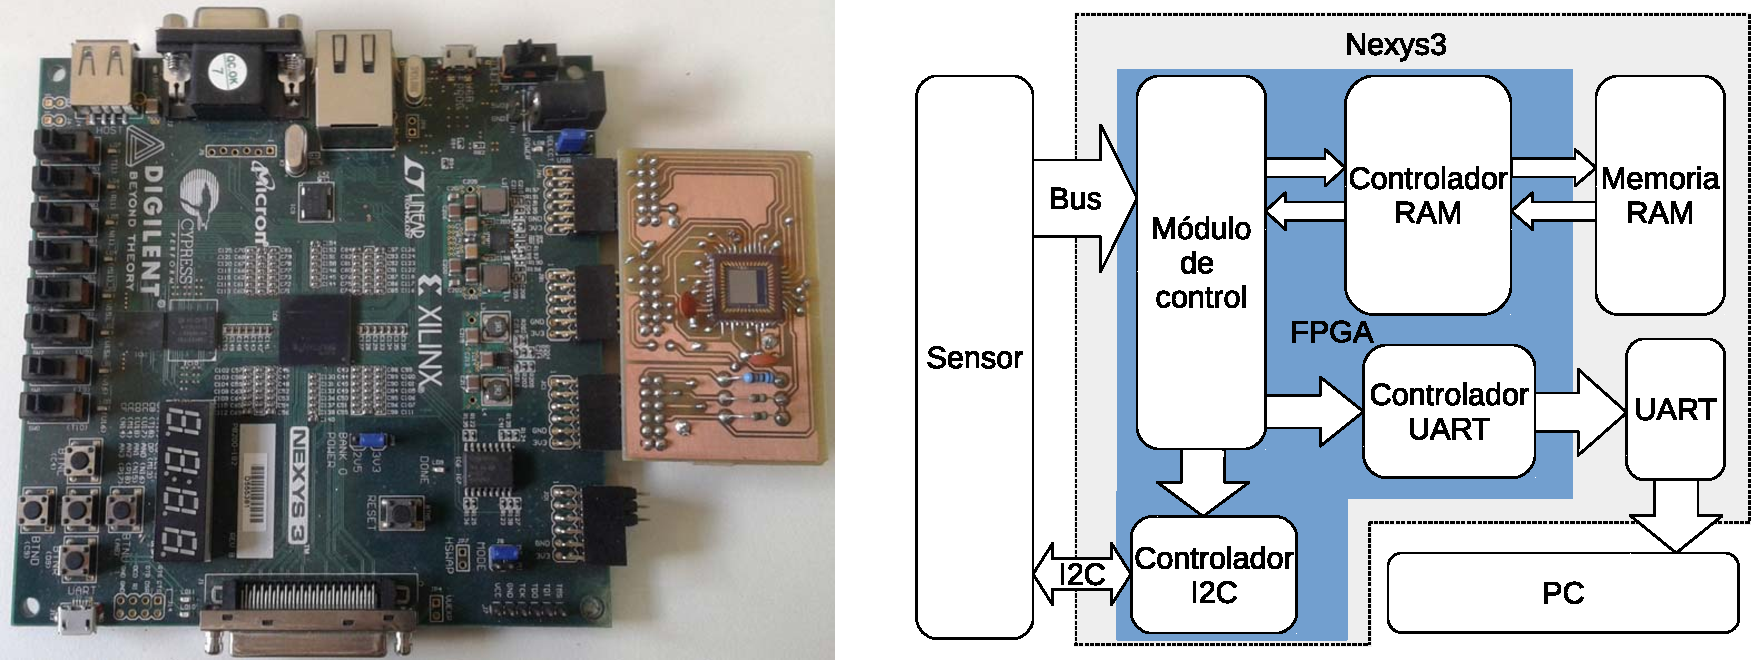
\includegraphics[width=0.9\paperwidth]{01motivacion}
	\end{frame}
	\begin{frame}{Agenda}
		\tableofcontents[hideallsubsections]
	\end{frame}
	\begin{frame}{Agenda}
		\tableofcontents[sections={1,2}]
	\end{frame}
	\begin{frame}{Agenda}
		\tableofcontents[sections={3,4}]
	\end{frame}
	\section{Introducción}
		\subsection{Motivación}
			\begin{frame}{La producción de información científica}
				
			\end{frame}
			\begin{frame}{La necesidad de una comunicación\\entre un FPGA y una PC}
				
			\end{frame}
		\subsection{Objetivos}
			\begin{frame}{Objetivos}
				\begin{itemize}
					\item
					\item
					\item
				\end{itemize}
			\end{frame}
		\subsection{Bus Serial Universal}
			\begin{frame}{USB - Bus Serial Universal}
				
			\end{frame}
	\section{Implementación}
		\subsection{Arquitectura del sistema}
			\begin{frame}{Arquitectura del sistema propuesto}
				
			\end{frame}
		\subsection{Configuración del puente}
			\begin{frame}{Firmware de configuración de la interfaz}
				
			\end{frame}
		\subsection{Circuito sintetizado}
			\begin{frame}{Interfaz puente - FPGA}
				
			\end{frame}
		\subsection{Circuito de interconexión}
			\begin{frame}{Circuito de interconexión}
				\begin{itemize}
					\item Versión 1
					\item Versión 2
					\item Version 3
				\end{itemize}
			\end{frame}
	\section{Evaluación y validación}
		\subsection{Test benchs de VHDL}
			\begin{frame}{Test Bench}
				
			\end{frame}
		\subsection{Depuración de firmware del puente}
			\begin{frame}{Debug Cypress}
				
			\end{frame}
		\subsection{Biblioteca de PC}
			\begin{frame}{\texttt{libusb-1.0}}
				
			\end{frame}
		\subsection{Programas de prueba}
			\begin{frame}{Esquemas de prueba}
				
			\end{frame}
		\subsection{Elementos de VHDL utilizados para depuración}
			\begin{frame}{Flip-Flop para eco}
				
			\end{frame}
			\begin{frame}{ROM con patrón de repetición infinita}
				
			\end{frame}
	\section{Resultados y conclusiones}
		\subsection{Robustez}
			\begin{frame}{Resultados de la prueba de robustez\\de la comunicación}
				
			\end{frame}
		\subsection{Tasa máxima de Transferencia}
			\begin{frame}{Resultados de la prueba de máxima transferéncia de datos}
				TODO
			\end{frame}
		\subsection{Trabajo futuro}
			\begin{frame}{Lo que falta...}
				
			\end{frame}
			\begin{frame}{Consultas}
				
			\end{frame}
			\begin{frame}[c]
				\centering
				\alert {Muchas gracias}
			\end{frame}
			
			\begin{frame}{Material Adicional}
				\centering
				Respaldo y cosas que no entren
			\end{frame}
\end{document}